\documentclass[conference]{IEEEtran}

% Packages
\usepackage[utf8]{inputenc}
\usepackage[english]{babel}
\usepackage{amsmath}
\usepackage{amsfonts}
\usepackage{amssymb}
\usepackage{amsthm}
\usepackage{pdfpages}
\usepackage{graphicx}
\usepackage{epstopdf}
\usepackage{listings}
\usepackage{cite}
\usepackage{enumerate}
\usepackage{scientific}
\usepackage[colorlinks=false]{hyperref}
\usepackage{bookmark}
\usepackage{paralist}

\usepackage[]{mcode}	%Matlab Code
\usepackage{tikz,pgfplots}	%Tikz

%\usepgfplotslibrary{external} 
%\tikzexternalize
%\tikzsetexternalprefix{ext/}

% Bookmark Setup
\bookmarksetup{numbered}

% PDF Setup
\hypersetup{pdftitle={Homework 7}, pdfsubject={Documentation of 7th Homework}, pdfauthor={Stefan Röhrl}, pdfkeywords={Neuroprothetik Exercise}, pdfcreator={LaTeX}, hidelinks}


\begin{document}
%
% cite all references
%\nocite{*}
%
% paper title
% can use linebreaks \\ within to get better formatting as desired
\title{Homework 7\\ CI Signalverarbeitung}

\author{\IEEEauthorblockN{Stefan Röhrl}
\IEEEauthorblockA{Technische Universität München, Arcisstraße 21, Munich, Germany\\
Email: stefan.roehrl@tum.de}}

% use for special paper notices
%\IEEEspecialpapernotice{(Invited Paper)}

% make the title area
\maketitle

\IEEEpeerreviewmaketitle

\section{Frequenzgang}
Beide Filterbänke teilen den Frequenzbereich von 200Hz bis 20.000Hz auf die verschiedenen Kanäle auf. Mit Butterworth Filtern kann man den Frequenzbereich in verschiedene Bänder aufteilen. Dies sind die Kanäle der Filterbank. Dass die Filter untereinander überlappen ist nicht ideal, jedoch müssen es realisierbare Filter sein, daher können diese nicht unendlich steile Flanken haben. Die 22-Kanal-Filterbank in Abb. \ref{fig:freq-gang-22} bietet eine wesentlich besser Aufteilung in kleine Frequenzbereiche, als die 3-Kanal-Filterbank in Abb. \ref{fig:freq-gang-3}. Somit ist zu erwarten, dass aus der 3-Kanal-Filterbank nicht so viel Informationen über die einzelnen Spektralanteile abgeleitet werden kann, wie von der 22-Kanal-Filterbank.
\begin{figure}[h]
	\vspace{-5pt}
	\centering
	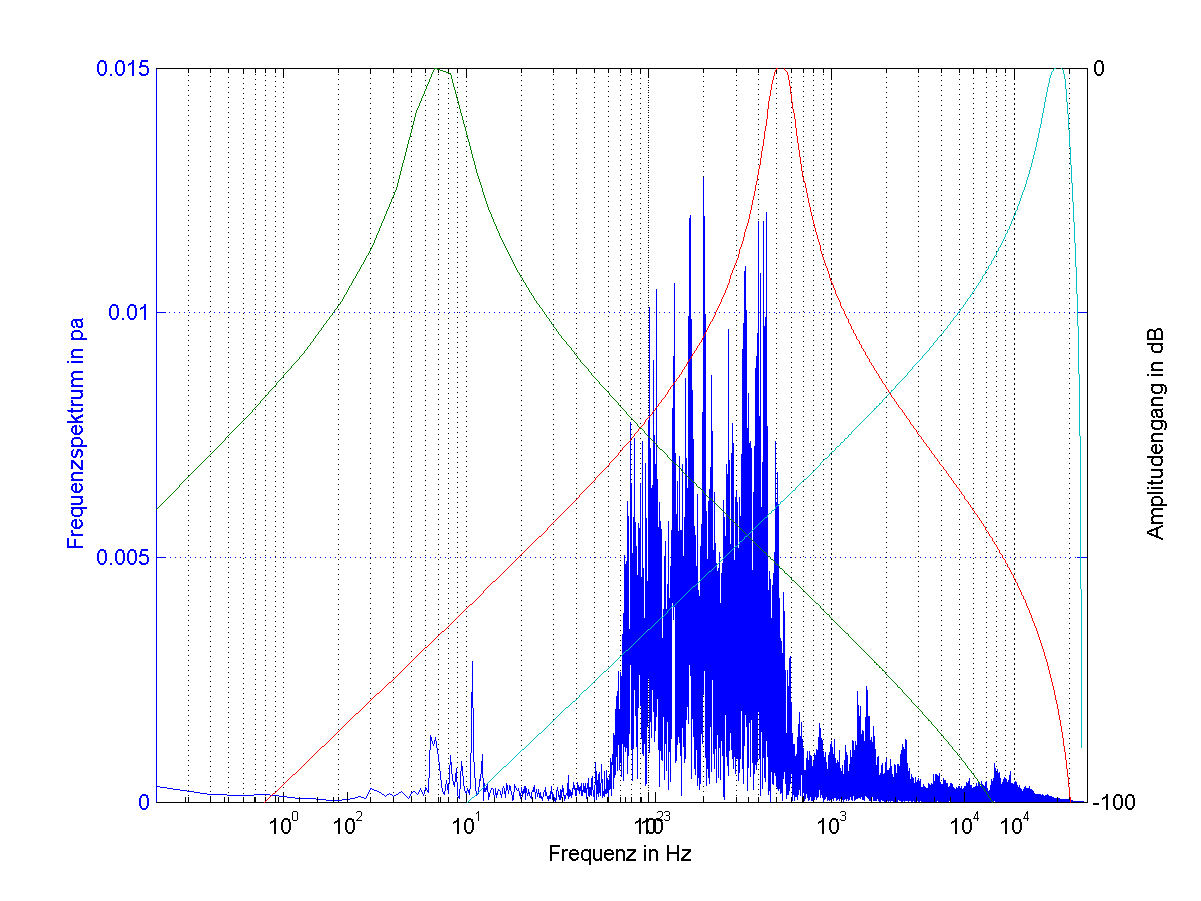
\includegraphics[width=0.45\textwidth]{img/freq_gang_3.png}
	\vspace{-10pt}
	\caption{Frequenzgang für 3 Kanäle}
	\vspace{-20pt}
	\label{fig:freq-gang-3}
\end{figure}

\begin{figure}[h]
	\vspace{-5pt}
	\centering
	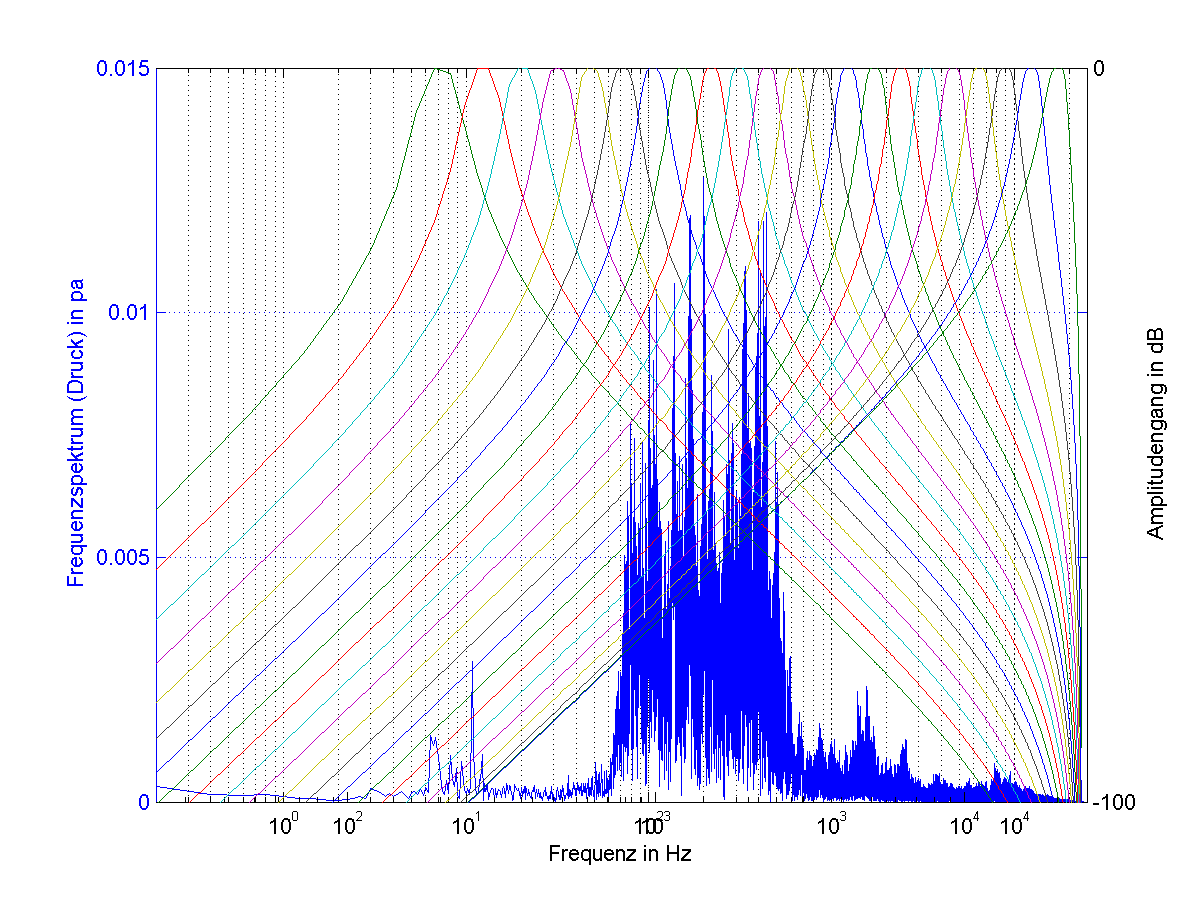
\includegraphics[width=0.45\textwidth]{img/freq_gang_22.png}
	\vspace{-10pt}
	\caption{Frequenzgang für 22 Kanäle}
	\vspace{-20pt}
	\label{fig:freq-gang-22}
\end{figure}

\section{Filterbank}
Die Signale die jeder Kanal ausgibt, sind in den Abbildungen \ref{fig:fb-6} und \ref{fig:fb-12} dargestellt. Wie im vorherigen Abschnitt erläutert steht jeder Kanal für ein bestimmtes Frequenzband. Somit sind im Ausgangssignal jedes Kanals fast nur Frequenzen enthalten, die dem Bereich des Kanals entsprechen. Die tiefsten Frequenzen sind in Kanal 1 zu finden, die höchsten in Kanal 6 bzw. 12. Daher sind z.B. Zischlaute mit hohen Frequenzen eher in den oberen Kanälen repräsentiert, als in den unteren. Dies entspricht einer Art Informationsvorverarbeitung. 
\begin{figure}[h]
	\vspace{-5pt}
	\centering
	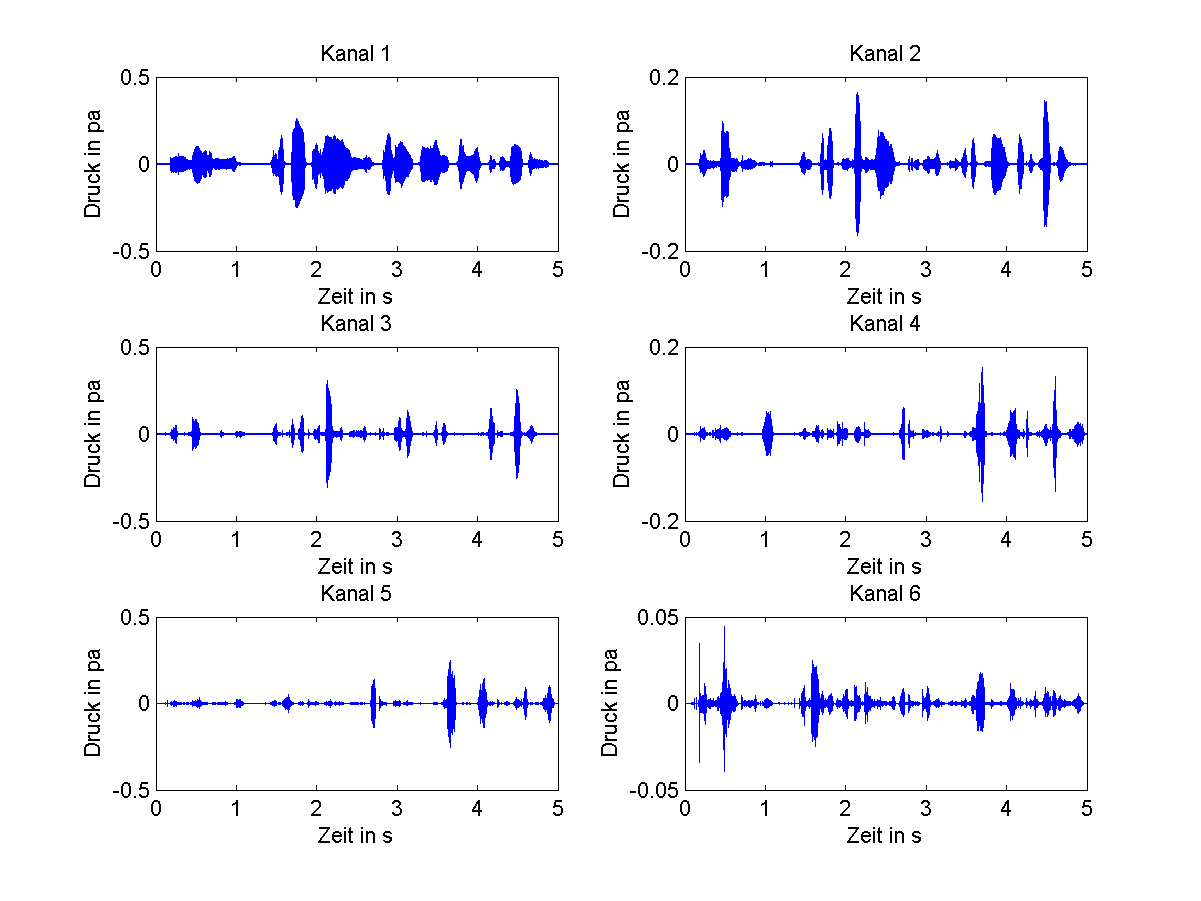
\includegraphics[width=0.5\textwidth]{img/fb_6.png}
	\vspace{-20pt}
	\caption{Gefilterte Signale mit 6 Kanälen}
	\vspace{-20pt}
	\label{fig:fb-6}
\end{figure}

\begin{figure}[h]
	\vspace{-5pt}
	\centering
	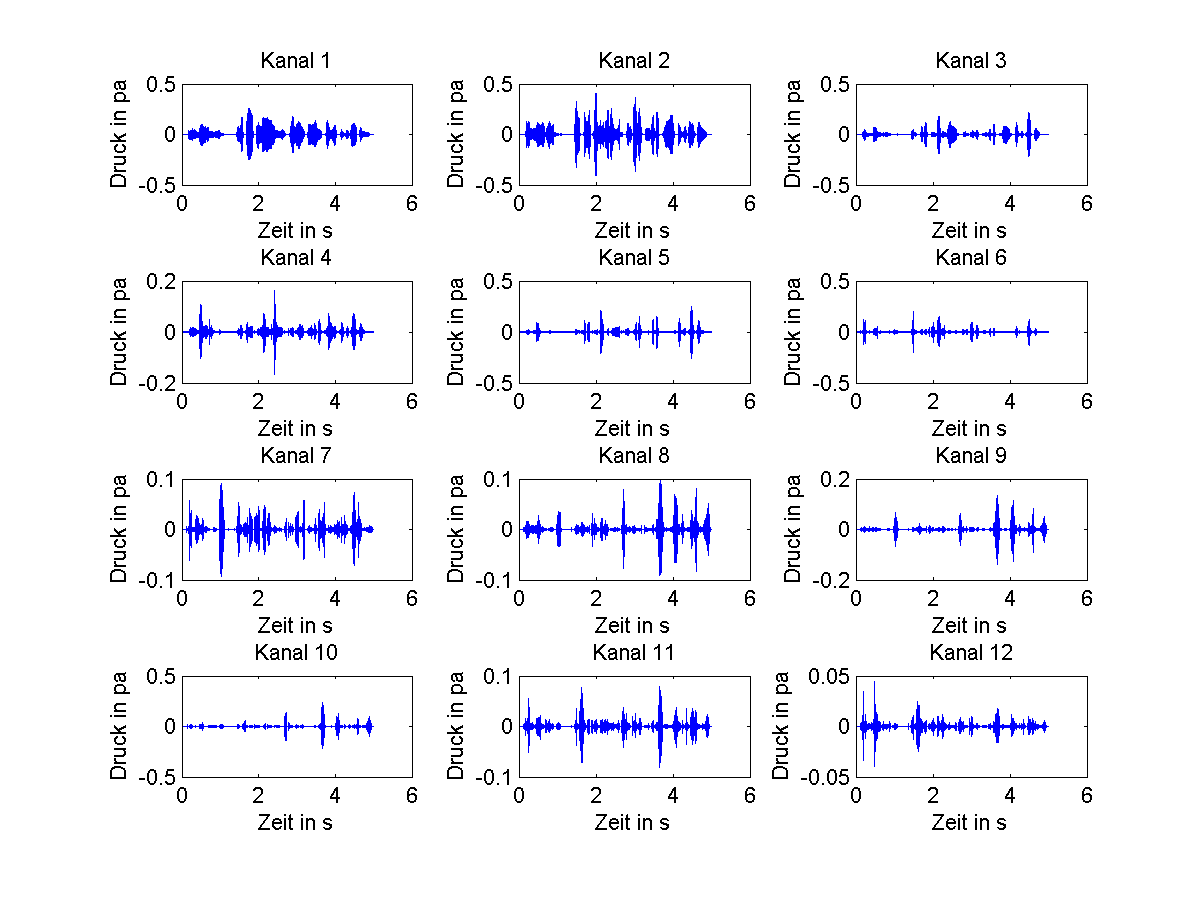
\includegraphics[width=0.5\textwidth]{img/fb_12.png}
	\vspace{-20pt}
	\caption{Gefilterte Signale mit 12 Kanälen}
	\vspace{-20pt}
	\label{fig:fb-12}
\end{figure}

\section{Kurzzeitspektrum}
\begin{compactenum}[a)]
\item Der Signalverlauf ist in allen Fällen relativ ähnlich. In Abbildung \ref{fig:sig-orig} ist das originale Signal dargestellt. In Abbildung \ref{fig:sig-rec-3} und \ref{fig:sig-rec-12} sind die Signale dargestellt die sich ergeben, wenn man die Antworten jedes Kanals wieder addiert, das Signal somit praktisch zu rekonstruieren versucht. Es ist leicht zu erkennen, dass das 12-Kanal-Signal mehr dem Original entspricht, als das 3-Kanal-Signal. 
\begin{figure}[h!]
	\vspace{-5pt}
	\centering
	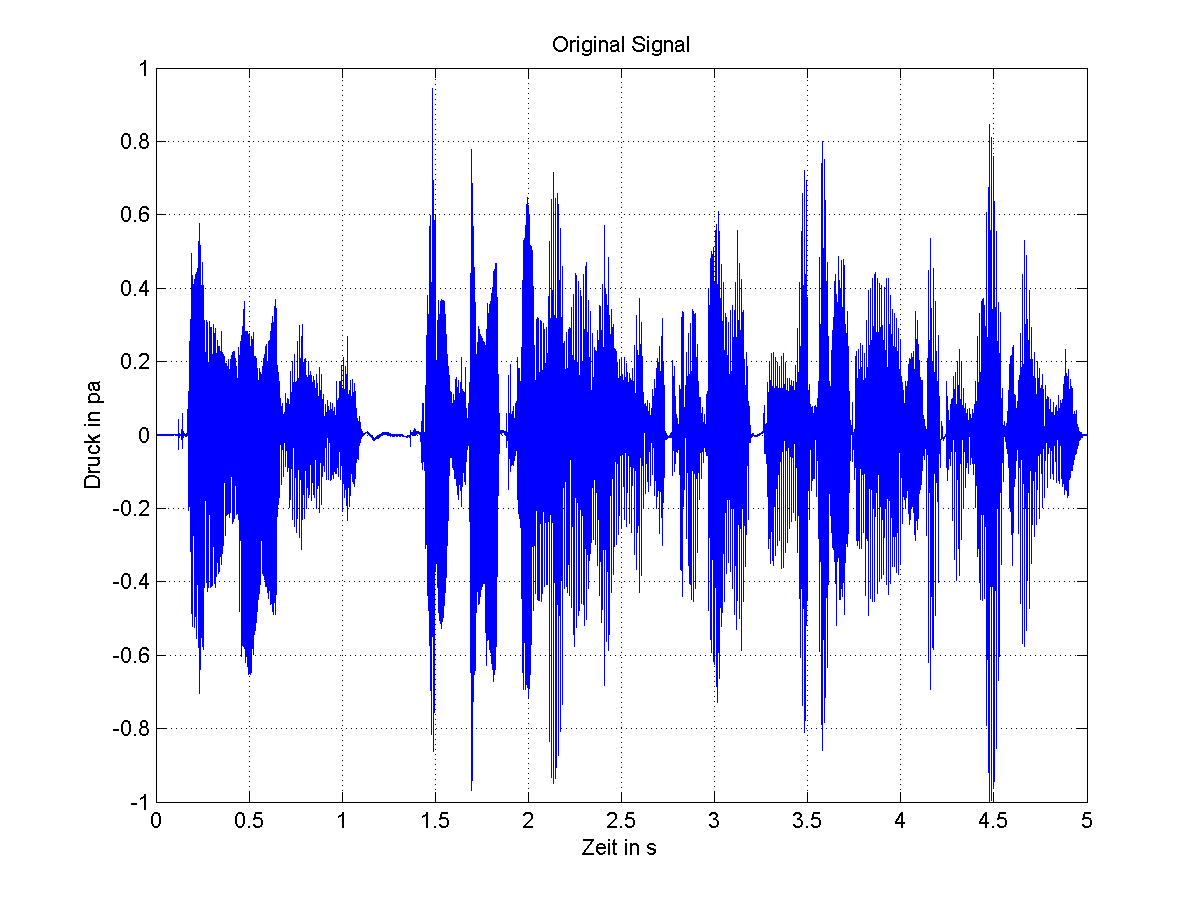
\includegraphics[width=0.4\textwidth]{img/sig_orig.png}
	\vspace{-10pt}
	\caption{Original Signal}
	\vspace{-10pt}
	\label{fig:sig-orig}
\end{figure}

\begin{figure}[h!]
	\vspace{-5pt}
	\centering
	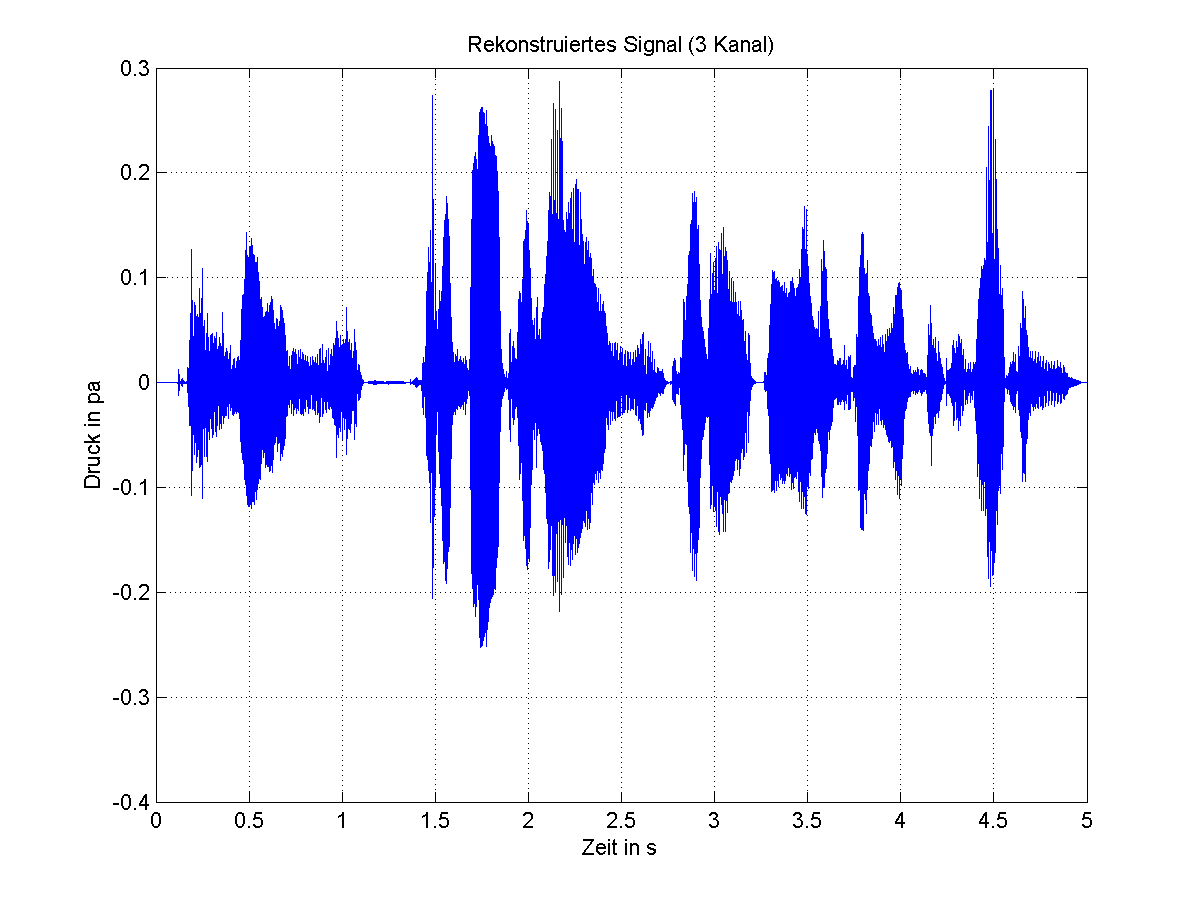
\includegraphics[width=0.4\textwidth]{img/sig_rec_3.png}
	\vspace{-10pt}
	\caption{Rekonstruiertes Signal von 3 Kanälen}
	\vspace{-10pt}
	\label{fig:sig-rec-3}
\end{figure}

\begin{figure}[h!]
	\vspace{-5pt}
	\centering
	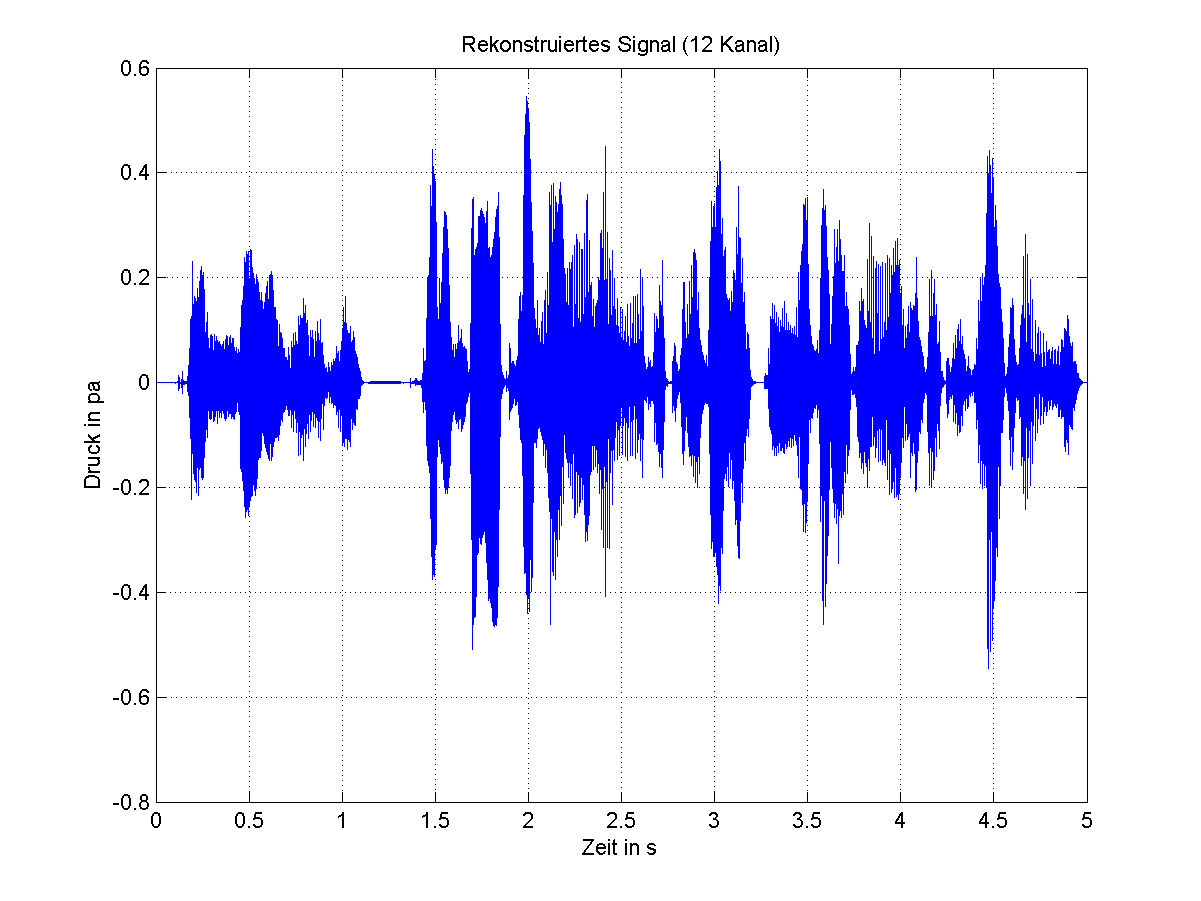
\includegraphics[width=0.4\textwidth]{img/sig_rec_12.png}
	\vspace{-10pt}
	\caption{Rekonstruiertes Signal von 12 Kanälen}
	\vspace{-10pt}
	\label{fig:sig-rec-12}
\end{figure}
\newpage
\item Der Unterschied in der Qualität der Filterbank mit mehr Kanälen wird besonders deutlich, wenn man sich die Spektren der wiederhergestellten Signale ansieht und sie mit dem Original vergleicht. Die 3-Kanal-Filterbank kann kaum den Dynamikumfang abbilden, den das gesprochene Signal hat. Das Spektrum sieht sehr zusammengestaucht und dünn aus. Man jedoch gut zwei der drei Bänder erkennen und in welchen Bereichen die Filter besonders durchlässige waren (vgl. Abb. \ref{fig:spect-rec-3}). Um ein qualitativ hochwertiges Signal zu haben, wäre es jedoch wünschenswert überhaupt keinen Filtereinfluss erkennen zu können. Daher empfiehlt es sich die 12-Kanal-Filterbank vorzuziehen, denn im zugehörigen Kurzzeitspektrum sieht man nur leicht das gewellte Muster, das von der Filterung stammt und die Bandpässe repräsentiert (vgl. Abb. \ref{fig:spect-rec-12}). Generell sieht dieses Kurzzeitspektrum dem Original wesentlich ähnlicher, obwohl es immer noch zu Fehlern kommt und die Rekonstruktion nicht verlustfrei ist. 
\begin{figure}[h!]
	\centering
	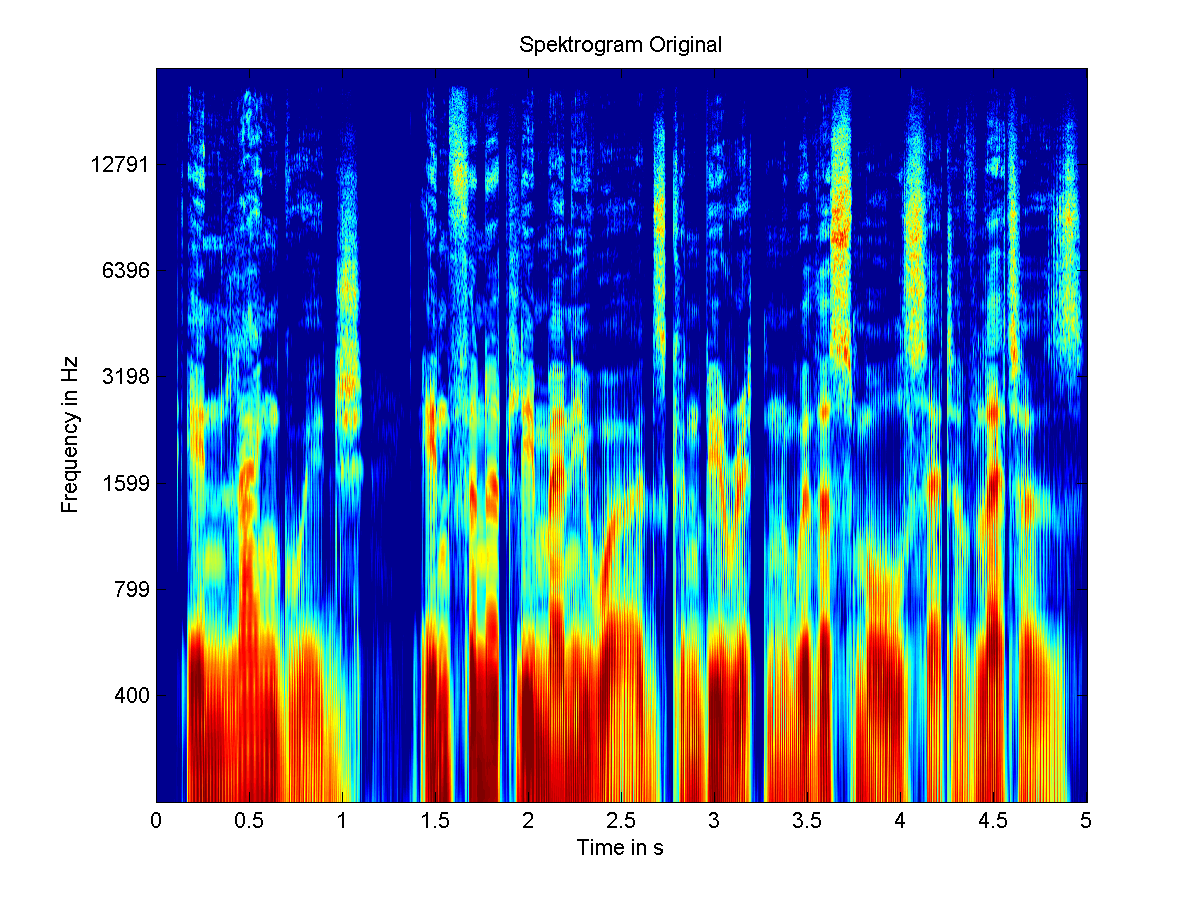
\includegraphics[width=0.5\textwidth]{img/spect_orig.png}
	\caption{Kurzzeitspektrum Original}
	\label{fig:spect-orig}
\end{figure}

\begin{figure}[h!]
	\centering
	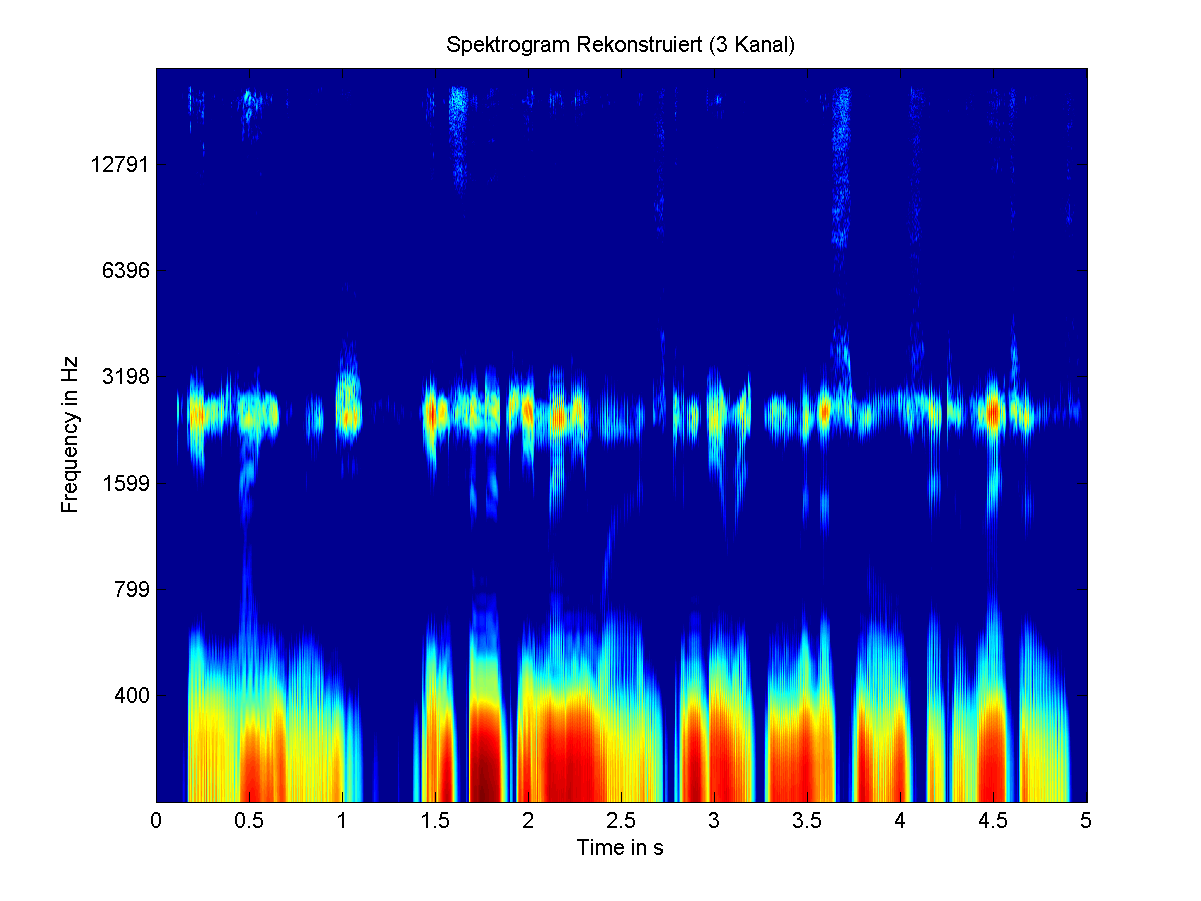
\includegraphics[width=0.5\textwidth]{img/spect_rec_3.png}
	\caption{Kurzzeitspektrum rekonstruiert von 3 Kanälen}
	\label{fig:spect-rec-3}
\end{figure}

\begin{figure}[h!]
	\centering
	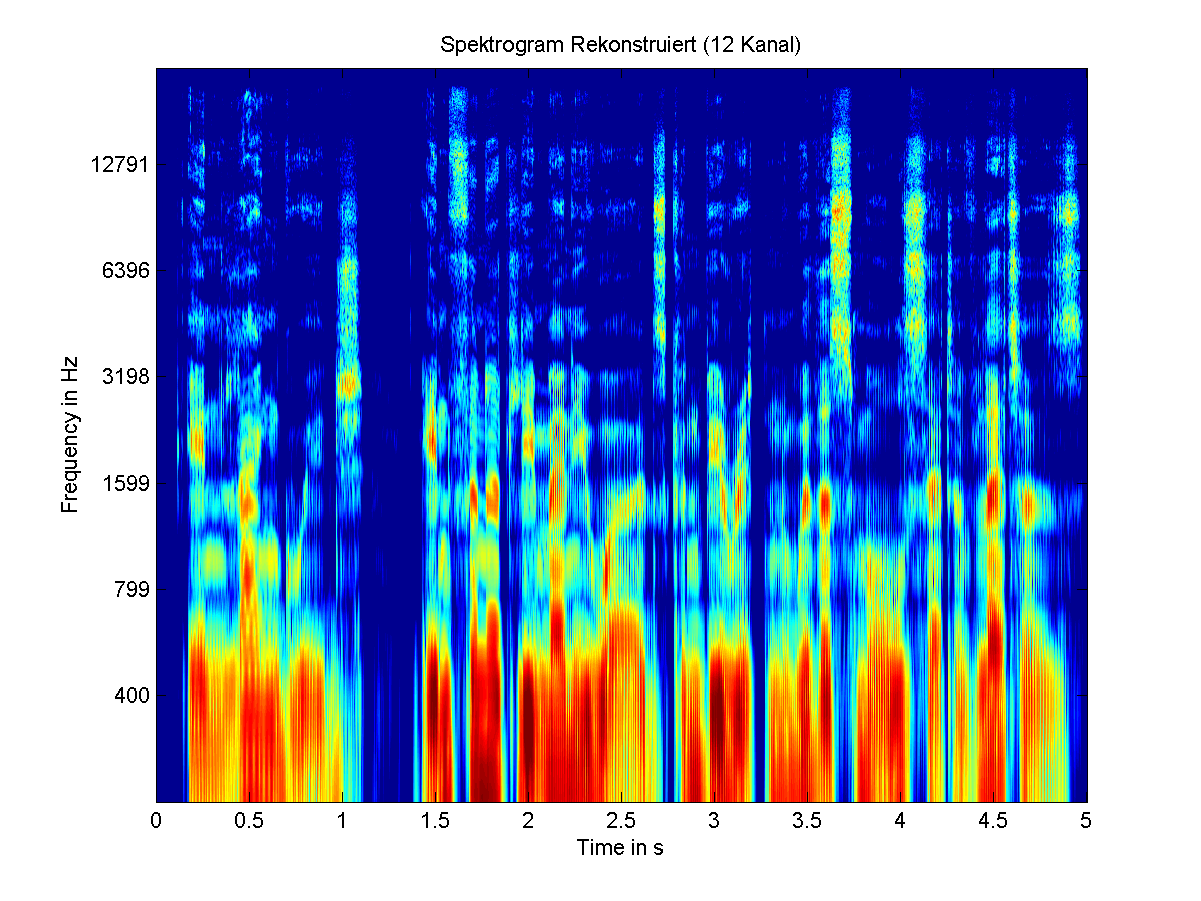
\includegraphics[width=0.5\textwidth]{img/spect_rec_12.png}
	\caption{Kurzzeitspektrum rekonstruiert von 12 Kanälen}
	\label{fig:spect-rec-12}
\end{figure}

\item Beim Langzeitspektrum der drei Signale lässt sich ähnliches erkennen. Man sieht deutlich, dass die 3-Kanal-Filterbank die enthaltenen Frequenzen deutlich ausdünnt und besonders den Sprach-Frequenzbereich stark einschränkt. Auch bei der 12-Kanal-Filterbank ist eine deutliche Dämpfung der Intensität erkennbar. Jedoch kann ein breiteres Spektrum abgebildet werden und man verliert nicht so viele Informationen. Die gewellte Form stammt wieder von den Maxima der Bandpassfilter jedes Kanals.
\begin{figure}[h!]
	\centering
	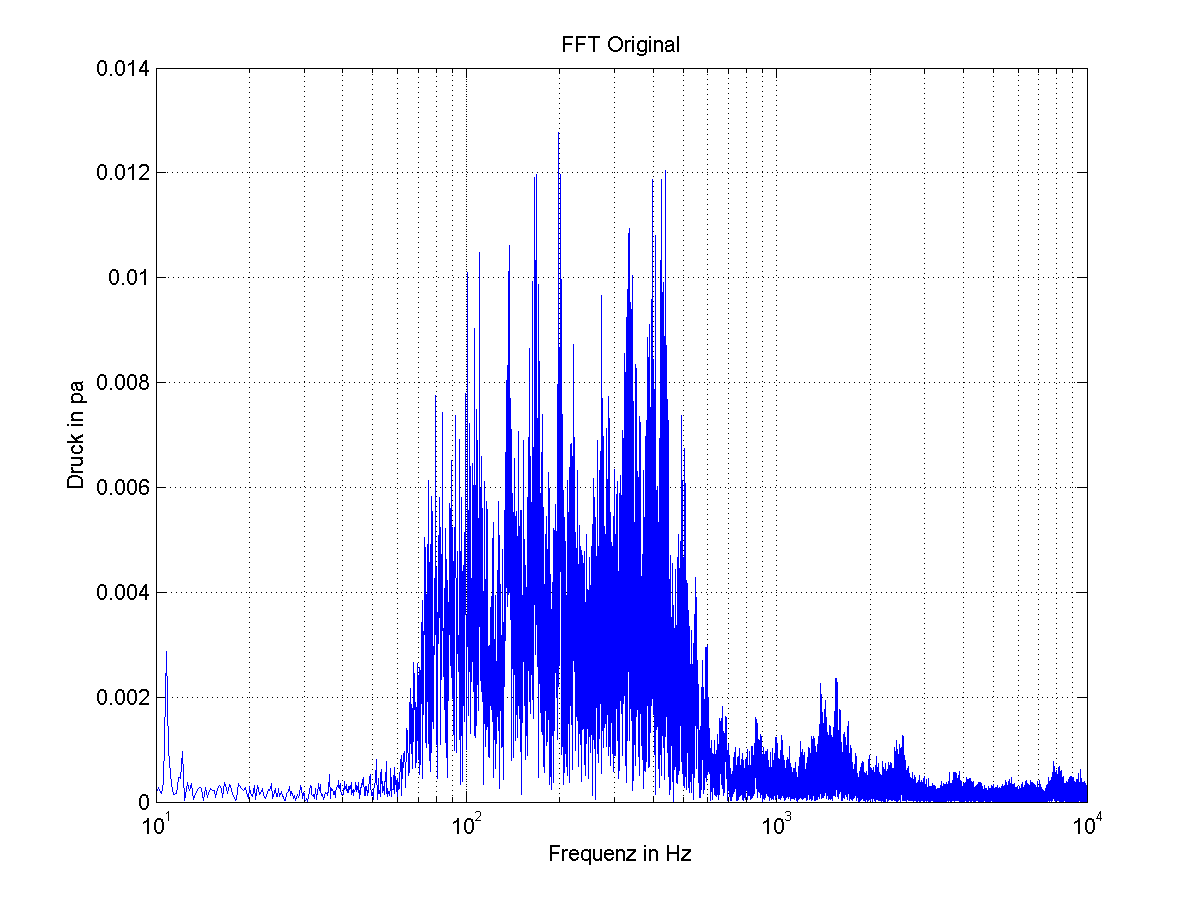
\includegraphics[width=0.5\textwidth]{img/fft_orig.png}
	\caption{Langzeitspektrum Original}
	\label{fig:fft-orig}
\end{figure}

\begin{figure}[h!]
	\centering
	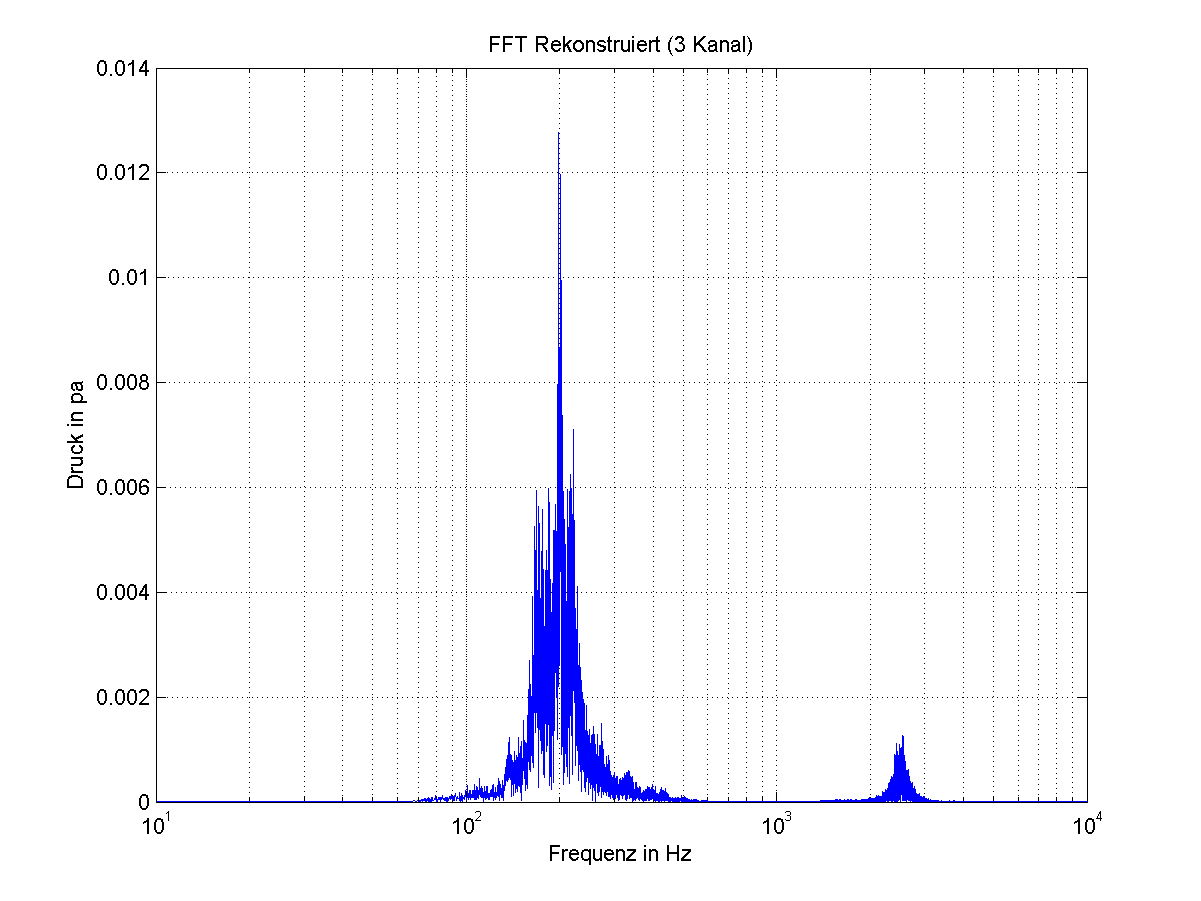
\includegraphics[width=0.5\textwidth]{img/fft_rec_3.png}
	\caption{Langzeitspektrum rekonstruiert von 3 Kanälen}
	\label{fig:fft-rec-3}
\end{figure}

\begin{figure}[h!]
	\centering
	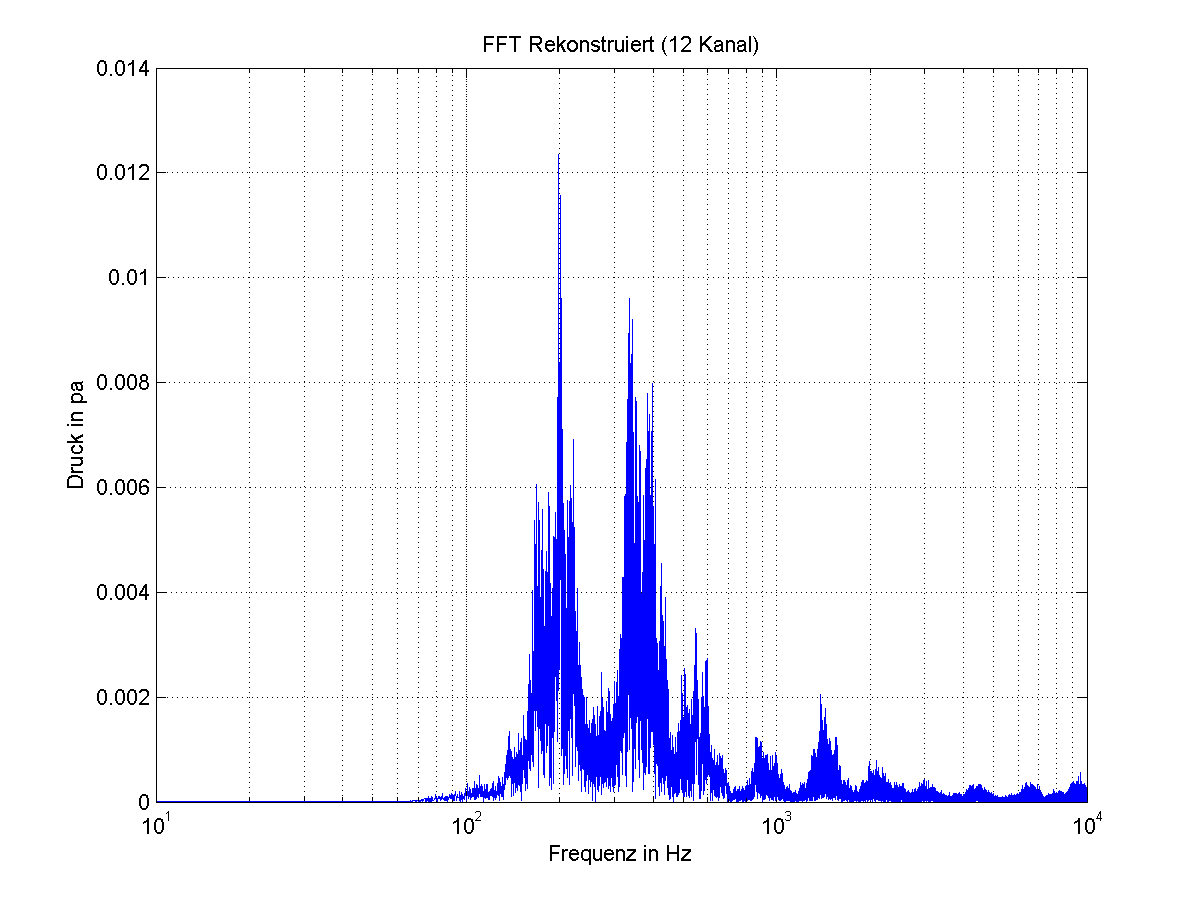
\includegraphics[width=0.5\textwidth]{img/fft_rec_12.png}
	\caption{Langzeitspektrum rekonstruiert von 12 Kanälen}
	\label{fig:fft-rec-12}
\end{figure}
\end{compactenum}



\end{document}


